\glsresetall
\chapter{Referencial Teórico}
\label{chap.background}

Neste capítulo serão apresentados alguns conceitos importantes para o entendimento do trabalho. Na Seção \ref{sec.lw} será apresentada uma visão geral de como os processadores evoluíram de \singlecores aos \lws. Na Seção \ref{sec.nanvixos} será apresentado o \so que será utilizado no desenvolvimento deste trabalho, o \nanvix. Na Seção \ref{sec.virtualizacao} será explicado um pouco sobre a virtualização e migração de processos, que é o tema principal do trabalho.

\section{Dos \singlecores aos \Lws}
\label{sec.lw}

Durante anos o aumento do desempenho dos processadores se manteve uma necessidade constante para o avanço da ciência em vários setores: astrologia, biologia, engenharia, etc. Até tempos atrás esse objetivo era alcançado através do aumento da frequência interna de \singlecores, do avanço na tecnologia dos semicondutores e do acréscimo do número de transistores em um \chip. Atualmente, estamos chegando a um limite físico que impede a aplicação dessas técnicas. Além da dificuldade de garantir o controle da dissipação de calor à medida que a frequência aumenta, o número de transistores que conseguimos colocar em um \chip está se estabilizando, haja vista o aparente impedimento na diminuição significativa do tamanho de um transistor.

Como alternativa para a continuidade nos avanços de poder computacional, foram exploradas novas técnicas. Em especial, foram desenvolvidas as arquiteturas paralelas, que exploram o poder de processamento paralelo, o qual é atingido pela execução de múltiplos \cores simultaneamtne. Essas novas arquiteturas são classificadas de acordo com a maneira com que conseguem manipular os dados. São elas:
\begin{inlinelist}
    \item \sisd;
    \item \simd;
    \item \misd;
    \item \mimd.
\end{inlinelist}
Neste trabalho, as mais relevantes são as arquiteturas que suportam cargas de trabalho \mimd, as quais ainda podem ser divididas em multiprocessadores ou multicomputadores, como mostrado na Figura \ref{fig.mimd} \cite{tanenbaum:4ed}. 

No presente trabalho, destaca-se a classe de processadores \lw, que pode ser classificada como \mpsoc. \Lws tem como objetivo atrelar o alto poder de processamento paralelo com eficiência energética. Para isso sua arquitetura segue as seguintes características:
\begin{enumerate}[label=(\roman*)]
    \item Integrar centenas ou milhares de núcleos de processamento operando a baixas frequências em um único chip;
    \item Operar sobre \mimd;
    \item Organizar os núcleos em conjuntos, denominados \clusters, para compartilhamento de recursos locais;
    \item Utilizar \nocs para transferência de dados entre núcleos ou \clusters;
    \item Possuir sistemas de memória distribuídos e restritivos, com pequenas memórias locais;
    \item Apresentar componentes heterogêneos (\cclusters e \ioclusters).
\end{enumerate}


\begin{figure}[bt]
    \centering
    \includesvg[width=0.9\linewidth]{content/images/mimd.svg}
    \caption{(a) um multiprocessador de memória compartilhada. (b) um multicomputator com troca de mensagens. (c) um sistema distribuído de grande escala.\cite{tanenbaum:4ed}}\label{fig.mimd}
\end{figure}

Alguns exemplos comerciais bem sucedidos de \lws são o \mppa \cite{dinechin:2013}, PULP \cite{pulp} e \taihulight \cite{fu2016sunway}. Uma visão conceitual da arquitetura de um \lw é ilustrada pela Figura \ref{fig.lw-overview}.

Mais detalhadamente, para o desenvolvimento deste trabalho será utilizado o processador \mppa. A Figura \ref{fig.arch-mppa} apresenta uma visão geral do processador e suas peculiaridades, tais como:

\begin{enumerate}[label=(\roman*)]
    \item integrar 288 núcleos de baixa frequência em um único chip;
    \item organizar os núcleos em 20 conjuntos (\clusters) para compartilhamento de recursos locais;
    \item utilizar 2 \nocs para transferência de dados entre \clusters;
    \item possuir um sistema de memória distribuída composto por pequenas memórias locais, \eg  \sram de 2 MB;
    \item não dispor de coerência de \cache;
    \item apresentar componentes heterogêneos, \eg \clusters destinados à computação ou comunicação com periféricos (\cclusters e \ioclusters, respectivamente).
\end{enumerate}

\begin{figure}[bt]
    \centering
    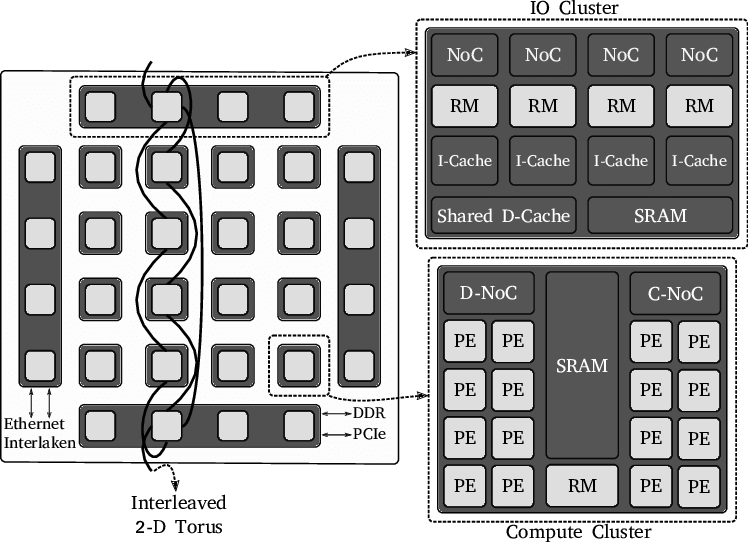
\includegraphics[width=0.6\linewidth]{content/images/arch-mppa-gs.png}
    \caption{Visão arquitetural do processador \mppa \cite{penna:sbesc19}}\label{fig.arch-mppa}
\end{figure}

\section{\nanvixos}\label{sec.nanvixos}

O \nanvix\footnote{Disponível em https://github.com/nanvix} é um \os distribuído e de propósito geral que busca equilibrar desempenho, portabilidade e programabilidade para \lws \cite{penna:sbesc19}. O \nanvix é estruturado em 3 camadas de \kernel. São elas:
\begin{description}
    \item [\nanvix \hal]
         é a camada mais baixa que abstrai e provê o gerenciamento dos recursos de \hardware sobre uma visão comum \cite{penna:hal}. Entre esses recursos estão: \cores, \tlbs, \cache, \mmu, \noc, interrupções, memória virtual, recursos de \io. De maneira geral, esta camada provê visões a nivel de \core, \cluster e comunicação/sincronização entre \clusters \cite{penna:thesis}. A Figura \ref{fig.hal-overview} ilustra a estrutura interna da \hal do \nanvix.
    \item [\nanvix \Assymetric \Microkernel]
        é a camada intermediária que provê gerenciamento de recursos e os serviços mínimos de um \os em um \cluster. Entre esses serviços se encontram a comunição intercluster, gerenciamento de \threads e memória, controle de acesso à memória e interface para chamadas de sistema. As chamadas de sistema podem ser executadas localmente, caso acessem dados \rdo ou alterem estruturas internas do \core, ou remotamente pelo \mcore, que atende à requisição e libera o \score requisitante ao seu término \cite{penna:thesis}. Essa característica adjetiva o \microkernel como assimétrico. A Figura \ref{fig.microkernel-overview} ilustra a estrutura interna do \microkernel do \nanvix.    
    \item [\nanvix \Multikernel]
        é a camada superior que provê os serviços de um \os e dispõe uma visão a nível do processador em si. Os serviços são hospedados em \clusters \ie isolados das aplicações de usuário e atendem as requisições vindas dos processos de usuário através de um modelo cliente-servidor. As requisições e respostas são enviadas/recebidas através de passagem de mensagem via \noc. Os serviços dessa camada podem ser entendidos como fontes de informação que mantém a execução dos processos consistentes no processador, tendo em vista a natureza distribuída da memória nessas arquiteturas. Nesses serviços estão incluídos mecanismos de \spawn de processos e obtenção de nomes lógicos dos processos (a fim de localizá-los para comunicação), por exemplo.
\end{description}

\begin{figure}[bt]
    \centering
    \includesvg[width=0.8\linewidth]{content/images/hal.svg}
    \caption{Estrutura interna da \hal do \nanvix \cite{penna:thesis}}\label{fig.hal-overview}
\end{figure}

\begin{figure}[bt]
    \centering
    \includesvg[width=0.8\linewidth]{content/images/microkernel.svg}
    \caption{Estrutura interna do \microkernel do \nanvix \cite{penna:thesis}}\label{fig.microkernel-overview}
\end{figure}

Em sua abordagem original, os processos no \nanvix são estáticos, \ie cada \cluster possui apenas um processo. Desse modo, uma vez que o processo inicia sua execução em um \cluster, este finalizará a execução no mesmo \cluster. 
Isso torna o processo dependente do \cluster que o executa \eg a comunicação entre processos está atrelada aos \clusters nos quais os processos são executados e não aos processos em si. A falta de mobilidade dos processos nesse modelo pode trazer sobrecargas ao processador e afeta o suporte a multi-aplicação. Por exemplo, a comunicação entre \clusters próximos é mais rápida e resulta em menor consumo energético do processador. Sendo assim, melhorar a mobilidade e a disposição dos processos no processador \ie viabilizar a migração de processos entre \clusters, possibilitaria melhorar o gerenciamento dos recursos do mesmo. Desse modo, este trabalho explora justamente essa dissassociação do \hardware com a execução do processo. Isso com o objetivo de desvincular o processo do \cluster que o executa, o que, por fim, aumentaria a mobilidade dos processos \ie a migração deles entre os \clusters.

\subsection{Abstrações de Comunicação do \nanvix}
O \nanvix dispõe de três abstrações de comunicações para transferência de dados e sincronização entre \clusters \cite{penna:thesis}. Nas próximas Seções serão detalhadas as três abstrações.

\begin{figure}[tb]
	\centering
	\subcaptionminipage[fig.sync1n]%
                   {.44\textwidth}
                   {Modo $1:N$.}
                   {\includesvg[width=\textwidth]{content/images/sync-1-n.svg}}
	\qquad
	\subcaptionminipage[fig.syncn1]
                   {.44\textwidth}
                   {Modo $N:1$.}
                   {\includesvg[width=\textwidth]{content/images/sync-n-1.svg}}
	\caption{Fluxo de execução da abstração \sync \cite{penna:thesis}.\label{fig.sync}}
\end{figure}

\subsubsection{\sync}
Esta abstração é a que da o suporte a sincronização inter-kernel. Através dela um processo pode esperar um sinal, que pode ser disparado por outro processo remotamente através das interfaces \noc. Essa abstração é muito utilizada na inicialização do sistema para garantia de sincronização entre os subsistemas \cite{penna:thesis}.

O \sync pode ser operado duas maneiras distintas: o modo $1:N$ e $N:1$. No modo $1:N$ (Figura \ref{fig.sync1n}) um nó envia uma notificação a múltiplos nós, que estão esperando pelo sinal. Em contraste, no moso $N:1$ (Figura \ref{fig.syncn1}), múltiplos nós enviam uma notificação a um único nó \cite{penna:thesis}.

\begin{figure}[bt]
    \centering
    \includesvg[width=0.5\linewidth]{content/images/mailbox.svg}
    \caption{Fluxo de execução da abstração \mailbox \cite{penna:thesis}}\label{fig.mailbox}
\end{figure}

\subsubsection{\mailbox}
Esta abstração é responsável pelo suporte à troca de mensagens de controle. Isso através de troca assíncrona de pequenas mensagens de tamanho fixo. A abstração segue a semântica $N:1$ e o funcionamento é o seguinte: um nó (destinatário da mensagem) possuí um \mailbox, do qual lê mensagens, e múltiplos nós (remetentes da mensagem) podem escrever nesse \mailbox \cite{penna:thesis}. A Figura \ref{fig.mailbox} ilustra o fluxo de execução da \mailbox.

\begin{figure}[b]
    \centering
    \includesvg[width=0.5\linewidth]{content/images/portal.svg}
    \caption{Fluxo de execução da abstração \portal \cite{penna:thesis}}\label{fig.portal}
\end{figure}

\subsubsection{\portal}
Esta abstração é reponsável pela troca de largas mensagens e segue a semântica $1:1$. A abstração pode ter uso em diversos cenários que exigem grandes transferências de dados entre \clusters \cite{penna:thesis}. A Figura \ref{fig.portal} ilustra o fluxo de execução da abstração \portal.
    

\section{Virtualização e Migração de Processos}
\label{sec.virtualizacao}

A virtualização pode ser entendida como a desvinculação da execução de uma aplicação (ou até um \so) dos recursos físicos responsáveis pelo seu funcionamento. O desacoplamento entre aplicação e \hardware, quando há virtualização, pode permitir, dependendo da camada em que esta é aplicada, a existência simultânea e isolada de múltiplas instâncias de usuários ou \oss (\vms), que compartilham e concorrem pelos mesmos recursos de \hardware reais. Reaproveitamento de recursos, portabilidade e segurança são algumas vantagens proporcionadas pela virtualização.

Em ambientes \cloud é muito comum a utilização de \vms para execução de tarefas nos servidores. Com o auxílio da virtualização, um único servidor pode alocar diversas \vms, possivelmente com \sos distintos. 

Neste trabalho, o foco é a virtualização de processos. Isto é, o objetivo é desacoplar a execução de uma aplicação do \cluster do \lw que a executa. Na abordagem original do \nanvix, o processo é dependente do local em que é alocado, o que afeta o suporte a migração e diminui a eficiência computacional, como detalhado na Seção \ref{sec.nanvixos}. Nesse contexto, a virtualização é útil justamente para aumentar a mobilidade dos processos, o que possibilitaria o gerenciamento da distribuição dos processos no processador. Particularmente, este trabalho trabalho explora um modelo mais leve de virtualização para \lw baseada em contêineres. Contêineres são executados pelo \os como aplicações virtuais e não incluem um \os convidado, resultando em um menor impacto no sistema de memória e requerendo menor complexidade do \hardware \cite{thalheim2018cntr, sharma2016containers}.